% !TEX root = file:///e:/thesis5sem/thesis.tex
\documentclass[14pt, a4paper]{extarticle}

\usepackage{listings}

\usepackage[paper=A4]{typearea}
\usepackage{lipsum}

\usepackage{caption}
\usepackage{graphicx}
\graphicspath{{./images/}}
\DeclareGraphicsExtensions{.jpg,.png}
\usepackage{csvsimple}

\usepackage{amsfonts}
\usepackage{amsmath}

\usepackage[english,russian]{babel}

\usepackage{fontspec} 
\usepackage{unicode-math}
\defaultfontfeatures{Ligatures={TeX},Renderer=Basic}
\setmainfont[Ligatures={TeX,Historic}]{Times New Roman}
\setmonofont{Courier New}
\setmathfont{XITSMath-Regular.otf}
\newfontfamily\cyrillicfonttt[Script=Cyrillic]{Courier New}
\babelfont{sf}{Droid Sans}
\numberwithin{equation}{section}

\usepackage{chngcntr}

\usepackage{xcolor}

\usepackage{array}
\newcommand\ChangeRT[1]{\noalign{\hrule height #1}}

\usepackage{tabularx}
\newcolumntype{s}{>{\raggedright\arraybackslash}X}
%\renewcommand{\tabularxcolumn}[1]{m{#1}} % Вертикальное центрирование текста

\usepackage{indentfirst} %отступ первой строки первого абзаца
\linespread{1.5}

\setlength{\footskip}{1cm}
\usepackage{geometry}
\geometry{left=3cm}
\geometry{right=1cm}
\geometry{top=2cm}
\geometry{bottom=2cm}

\setlength{\parindent}{1.25cm}

\usepackage{enumitem}
\setlist{left=\parindent, labelsep=1cm, itemsep=0pt, topsep=0pt}

\usepackage[final]{pdfpages}

\usepackage{titlesec} % оформление заголовков

\titleformat{\section}[block]
	{\bfseries\fontsize{18pt}{21.6pt}\selectfont}
        {\thesection}
        {1em}{}
\titleformat{name=\section,numberless}[block]
	{\centering\bfseries\fontsize{18pt}{21.6pt}\selectfont}
        {}
        {0em}{}{}
\titlespacing{\section}
 {\parindent}% space at the left
 {0em}% space before
 {10mm}% space after
\titleformat{\subsection}[block]
	{\bfseries\hspace{\parindent}\fontsize{16pt}{19.2pt}\selectfont}
        {\thesubsection}
        {1em}{}

% Отображать только заголовки первого уровня
%\setcounter{tocdepth}{1}

\usepackage{etoolbox}

\usepackage{nameref}

\usepackage{xurl}
\usepackage{hyperref}
\hypersetup{
    colorlinks,
    citecolor=black,
    filecolor=black,
    linkcolor=black,
    urlcolor=black,
    breaklinks=true
}
\urlstyle{same}
       
\usepackage{float}
\usepackage{graphicx,kantlipsum,setspace}

\usepackage{newfloat}
\DeclareCaptionType[name=Листинг, placement=htbp]{listing}

\usepackage{fancyvrb}

\DeclareCaptionLabelSeparator{emdash}{\;\textemdash\;}
\captionsetup[figure]{name={Рисунок}, 
                      labelsep=emdash, 
                      justification=centering, 
                      position=above, 
                      singlelinecheck=off, 
                      font={singlespacing, small, bf},
                      labelfont=bf, 
                      skip=6pt}

\captionsetup[table]{name={Таблица}, 
                     labelsep=emdash, 
                     justification=raggedright, 
                     position=top, 
                     singlelinecheck=off, 
                     font={singlespacing, small, it}, 
                     labelfont=it, 
                     skip=0pt, 
                     margin=0cm}

\captionsetup[lstlisting]{labelsep=emdash, 
                          justification=raggedright, 
                          position=top, 
                          singlelinecheck=off, 
                          font={singlespacing, small, it}, 
                          labelfont=it, 
                          skip=0pt, 
                          margin=0cm}


% Нумерация по разделам
\counterwithin{figure}{section}
\counterwithin{table}{section}
\counterwithin{listing}{section}

\usepackage{ragged2e}
\usepackage{microtype}

\justifying
\tolerance=500
\hyphenpenalty=10000 % отключение переноса
\emergencystretch=3em

\usepackage{setspace}

\usepackage{multirow}

\usepackage[
citestyle=gost-numeric,
style=gost-numeric, 
blockpunct=emdash,
backend=biber,
sorting=none
]{biblatex}

\defcounter{biburlnumpenalty}{3000}
\defcounter{biburlucpenalty}{6000}
\defcounter{biburllcpenalty}{9000}

\DeclareFieldFormat{url}{Режим доступа: #1}
\DeclareFieldFormat{urldate}{(Дата обращения: #1)}
\renewcommand*{\entrysetpunct}{\par\nopunct\!\!}


\defbibheading{bibliography}[\bibname]{%
  \section*{\centering #1}%
  \markboth{#1}{#1}}


\usepackage{pdflscape}
\usepackage{everypage}

\newcommand{\Lpagenumber}{\ifdim\textwidth=\linewidth\else\bgroup
  \dimendef\margin=0 %use \margin instead of \dimen0
  \ifodd\value{page}\margin=\oddsidemargin
  \else\margin=\evensidemargin
  \fi
  \raisebox{\dimexpr-\topmargin-\headheight-\headsep-0.5\linewidth}[0pt][0pt]{%
    \rlap{\hspace{\dimexpr-\margin+\textheight+\footskip}%
    \llap{\rotatebox{90}{\thepage}}}}%
\egroup\fi}
\AddEverypageHook{\Lpagenumber}%

\usepackage{tocloft}
\setlength{\cftsecnumwidth}{0pt}
\setlength{\cftsecindent}{0pt}% Remove indent for \section
\setlength{\cftsubsecindent}{0pt}% Remove indent for \subsection
\setlength{\cftsubsubsecindent}{0pt}% Remove indent for \subsubsection
\setlength{\cftbeforesecskip}{0pt}% Change spacing between sections
\renewcommand{\cftsecaftersnumb}{\hspace{1.5em}}
\renewcommand{\cftsecleader}{\cftdotfill{\cftdotsep}}
\renewcommand{\cftdotsep}{1.25}
\renewcommand{\cftsecfont}{\normalfont}
\renewcommand{\cftsecpagefont}{\normalfont}
\renewcommand{\cfttoctitlefont}{\hfil \bfseries \large}

% Поддержка листингов
\usepackage{listings}
\lstdefinestyle{gost}{
    basicstyle=\ttfamily\fontsize{10pt}{10pt}\linespread{1}\selectfont,
    breakatwhitespace=false,
    breaklines=true,
    keepspaces=true,
    showspaces=false,          
    showstringspaces=false,
    frame=single
}
\lstset{style=gost}

\addbibresource{thesis.bib}

\usepackage{lipsum} 


\begin{document}

\counterwithin{lstlisting}{section}

\pretocmd{\section}{\newpage}{}{}

\def\contentsname{СОДЕРЖАНИЕ}

\pagenumbering{gobble}
\begin{titlepage}

\includepdf[pages=-]{title/ivbo-06-21_гостев}
\end{titlepage}
\tableofcontents

\section*{ВВЕДЕНИЕ}
\pagenumbering{arabic}
\setcounter{page}{4}

%%% Актуальность, Важность исследования
В современном мире, где темпы технологического прогресса 
неуклонно растут,  роль информационных технологий (ИТ) в 
бизнес-сфере становится всё более значимой. 
Интеграция ИТ в бизнес-процессы предприятия способствует 
увеличению общей эффективности и производительности бизнеса. 
Как показывают исследования, "революция ИТ и интернета 
способствует выдающимся результатам в экономике 
бизнес-сектора через обмен информацией с использованием 
интернета и электронных устройств, 
облегчая доступность ведения бизнеса между компаниями на 
глобальном уровне"\cite{mgunda2019impacts}.
Построение качественной сети передачи данных и современных 
серверных служб для предприятия, 
является важной задачей, решение которой позволит улучшить 
эффективность работы предприятия 
и качество обслуживания клиентов.
Это показывает, насколько критично для современных 
предприятий интегрировать современные информационные 
технологии в свои процессы, чтобы оставаться 
конкурентоспособными на рынке.

%%% Объект, предмет, цель
Объектом данного исследования является сеть передачи данных, предприятия, 
а предметом - особенности проектирования и реализации сети передачи данных. 
Целью работы является планирование и реализация качественной, гибкой и 
эффективной сети передачи данных для предприятия, осуществляющего розничную 
торговлю изделиями, применяемыми в медицинских целях, в специализированных магазинах.

%%% Задачи

%%% Методы исследования
В ходе проведения исследования будет использован ряд методов. 
Метод моделирования будет использован для создания и тестирования 
модели сети,  что обеспечит возможность визуализации предполагаемых 
результатов до их реализации. Метод аналогии будет служить инструментом 
сравнения различных моделей сетей,  что позволит определить наиболее 
подходящий вариант для конкретного предприятия. При помощи метода 
классификации будут описаны и рассмотрены различные площадки, 
такие как главный штаб, склады и филиалы, а также соответствующие им сети. 
Метод изучения и анализа литературы обеспечит знакомство 
с существующими решениями и теоретическими знаниями в области 
проектирования сетей передачи данных.



%%% Источники информации
Основными источниками информации 
для данной работы станут научные статьи, 
учебники по теме "Технологии передачи данных", 
включая книгу Олифера "Сети", 
а также документация и руководства по работе 
с модулями Cisco и программой 
Cisco Packet Tracer. Также будет использована 
информация с ресурса Habr, 
где представлены актуальные статьи и обзоры 
по теме сетевых технологий.

%%% Интсрументальные средства
В процессе выполнения работы будет применён ряд 
инструментальных средств. 
Программное обеспечение для моделирования сетей Cisco 
Packet Tracer будет использовано для проектирования 
и тестирования сети. Это обеспечит точное 
воссоздание планируемых сетевых структур и их 
тестирование в контролируемых условиях. 
Для обеспечения эффективного разделения сети на 
подсети будет использован калькулятор IP-сетей. 
Это инструмент позволит оптимизировать процесс 
разбиения сети на подсети, ускорив его и 
снизив вероятность ошибок. Веб-сервисы с сайта 
diagrams.net будут использованы для построения 
топологий сети и различных диаграмм. 
Это обеспечит наглядность представления 
структуры сети и связей между её элементами.

%%% Содержание работы

\section{ПЛАНИРОВАНИЕ И ПРОЕКТИРОВАНИЕ СЕТИ ПЕРЕДАЧИ ДАННЫХ}

\subsection{Определение структуры предприятия}
Предприятие, являющееся объектом проектирования сети, обладает многоуровневой 
комплексной структурой, состоящей из разнообразных подразделений и отделов. 
Визуализация организационного строения компании способствует выявлению и устранению
неэффективных компонентов в её структуре, а также наглядному представлению структурных
особенностей предприятия, что может являться полезным при проектировании сети передачи
данных.


Методолгия ARIS предоставляет удобные и результативные 
способы визуализации и анализа организационной структуры компании. На Рисунках 
\ref{fig:mainDepartamentStructure}-\ref{fig:warehouseStructure} представлены
организационные структуры для каждого объекта предприятия: главного штаба, филиала, точки присутствия и склада. Структуры выполнены в соответствии с методологией ARIS.

\begin{figure}[H]
        \centering
        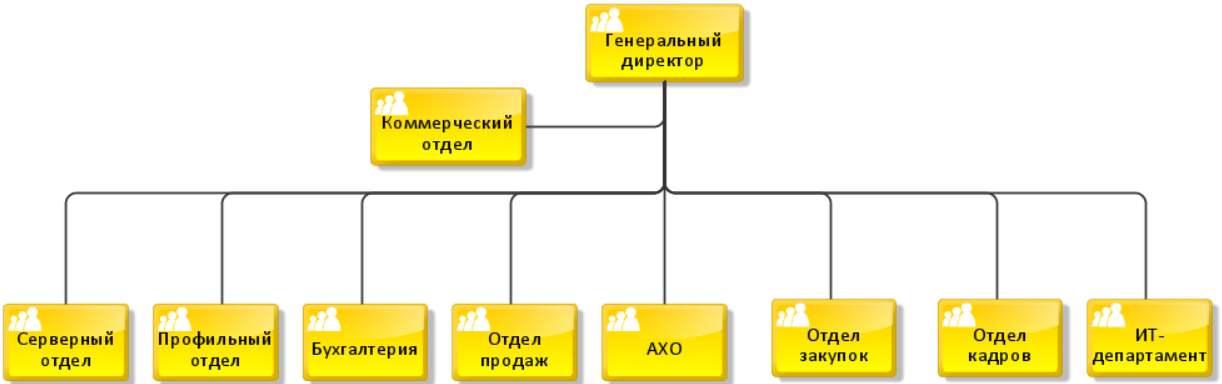
\includegraphics[scale=0.6]{ARIS_mainDepStructure.png}
        \caption{Организационная структура главного штаба}
        \label{fig:mainDepartamentStructure}
\end{figure}

\begin{figure}[H]
        \centering
        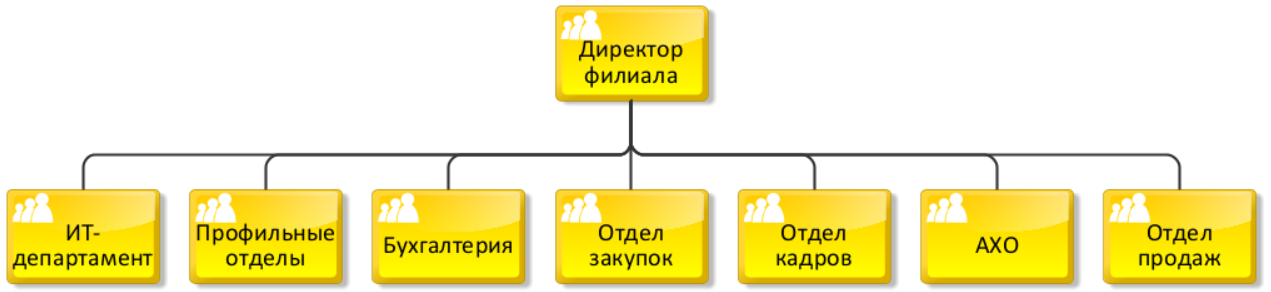
\includegraphics[scale=0.6]{ARIS_filialStructure.png}
        \caption{Организационная структура филиала}
        \label{fig:filialStructure}
\end{figure}

\begin{figure}[H]
        \centering
        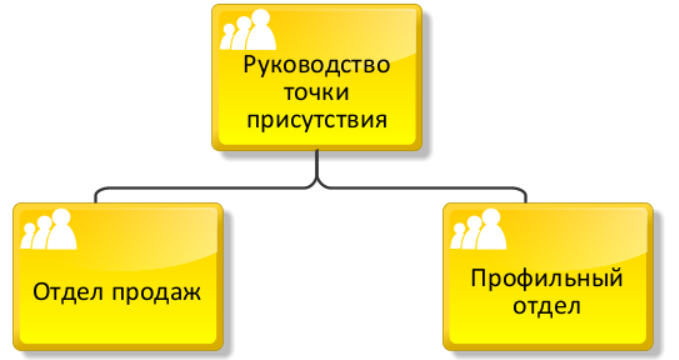
\includegraphics[scale=0.6]{ARIS_tpStructure.png}
        \caption{Организационная структура точки присутствия}
        \label{fig:tpStructure}
\end{figure}

\begin{figure}[H]
        \centering
        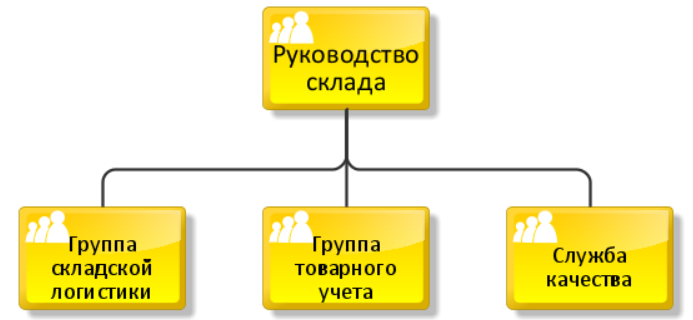
\includegraphics[scale=0.6]{ARIS_warehouseStructure.png}
        \caption{Организационная структура склада}
        \label{fig:warehouseStructure}
\end{figure}

Для полноценного анализа структуры предприятия необходимо учитывать не 
только численность персонала по отделам, но и количество АРМ, 
соответствующих потребностям сотрудников. В большинстве отделов число 
АРМ равно числу работников, за исключением административно-хозяйственной 
службы с посменной работой и группы складской логистики, где АРМ не требуются. 
Данные по количеству сотрудников и АРМ представлены в Таблицах 
\ref{table:mainDepPopul}-\ref{table:warehousePopul}.

\begin{table}[H]
\centering
\small
\caption{Численность персонала в главном штабе}
\begin{tabular}{|m{5cm}|m{3cm}|m{3cm}|}
\hline
\textbf{Название отдела} & \textbf{Количество людей} & \textbf{Количество АРМ} \\
\hline
Руководство предприятия & 1 & 1 \\
\hline
Коммерческий отдел & 3 & 3 \\
\hline
Бухгалтерия & 10 & 10 \\
\hline
Отдел кадров & 20 & 20 \\
\hline
Отдел закупок & 30 & 30 \\
\hline
Отдел продаж & 55 & 55 \\
\hline
Административно-хозяйственная служба & 15 & 2 \\
\hline
ИТ-департамент & 20 & 20 \\
\hline
Профильные отделы & 45 & 45 \\
\hline
Серверный отдел & 1 & 1 \\
\hline
\end{tabular}
\label{table:mainDepPopul}
\end{table}


\begin{table}[H]
\centering
\small
\caption{Численность персонала в филиале}
\begin{tabular}{|m{5cm}|m{3cm}|m{3cm}|}
\hline
\textbf{Название отдела} & \textbf{Количество людей} & \textbf{Количество АРМ} \\
\hline
Руководство предприятия & 1 & 1 \\
\hline
Бухгалтерия & 5 & 5 \\
\hline
Отдел кадров & 10 & 10 \\
\hline
Отдел закупок & 10 & 10 \\
\hline
Отдел продаж & 10 & 10 \\
\hline
Административно-хозяйственная служба & 5 & 2 \\
\hline
ИТ-департамент & 10 & 10 \\
\hline
Профильные отделы & 19 & 19 \\
\hline
\end{tabular}
\label{table:filialPopul}
\end{table}


\begin{table}[H]
\centering
\small
\caption{Численность персонала в точке присутствия}
\begin{tabular}{|m{5cm}|m{3cm}|m{3cm}|}
\hline
\textbf{Название отдела} & \textbf{Количество людей} & \textbf{Количество АРМ} \\
\hline
Руководство точки присутствия & 1 & 1 \\
\hline
Отдел продаж & 2 & 2 \\
\hline
Профильный отдел & 3 & 3 \\
\hline
\end{tabular}
\label{table:tpPopul}
\end{table}


\begin{table}[H]
\centering
\small
\caption{Численность персонала на складе}
\begin{tabular}{|m{4cm}|m{3cm}|m{3cm}|}
\hline
\textbf{Название отдела} & \textbf{Количество людей} & \textbf{Количество АРМ} \\
\hline
Руководство склада & 2 & 2 \\
\hline
Группа складской логистики & 5 & 1 \\
\hline
Группа товарного учета & 13 & 13 \\
\hline
Служба качества & 10 & 10 \\
\hline
\end{tabular}
\label{table:warehousePopul}
\end{table}


\subsection{Расчёт пропускной способности каналов передачи данных}
В данном пункте следует произвести расчет пропускной способности каналов передачи 
данных с учетом применения трехуровневой архитектуры сети, состоящей 
из уровня доступа, агрегации и ядра. 

Расчеты по количеству портов выполняются следующим образом.
На уровне доступа количество портов соответствует количеству терминалов 
с проводным подключением. 
Чтобы рассчитать количество портов на уровне агрегации, необходимо 
учесть коэффициент перехода от уровня доступа, обусловленный тем, 
что конечные узлы не используют весь канал передачи данных на 
постоянной основе и активные приложения не сильно 
чувствительны к задержкам и потерям. Выяснено, что такой коэффициент равен 0.4,
Для уровня ядра требуется соотношение один к одному для пропускной способности канала.
Также необходимо определить скоростные требования
к портам для пользователей: обычным пользователям выделяется 
100 МБит/с, руководящим должностям выделяется 1 ГБит/с, так как 
бесперебойное и надежное соединение в 
этом случае крайне необходимо, учитывая постоянные 
переговоры, использующие интернет-соединение, серверный отдел 
использует полный предлагаемый трафик в 1 ГБит/с. 

В Таблице \ref{table:mainDepAccessLevel} представлены расчеты портов для уровня доступа 
главного штаба.

\begin{table}[H]
\centering
\small
\caption{Расчет портов уровня доступа для главного штаба}
\begin{tabular}{|m{4cm}|m{2.5cm}|m{2.5cm}|m{2.5cm}|m{3cm}|}
\hline
\textbf{Название отдела} & \textbf{Количество АРМ} & \textbf{Требования к скорости, Мбит/с} & \textbf{Кол-во портов FastEthernet} & \textbf{Кол-во портов GigabitEthernet} \\
\hline
Руководство предприятия & 1 & 1000 & 0 & 1 \\
\hline
Коммерческий отдел & 3 & 1000 & 0 & 3 \\
\hline
Бухгалтерия & 10 & 100 & 10 & 0 \\
\hline
Отдел кадров & 20 & 100 & 20 & 0 \\
\hline
Отдел закупок & 30 & 100 & 30 & 0 \\
\hline
Отдел продаж & 55 & 100 & 55 & 0 \\
\hline
Административно-хозяйственная служба & 2 & 100 & 2 & 0 \\
\hline
ИТ-департамент & 20 & 100 & 20 & 0 \\
\hline
Профильные отделы & 45 & 100 & 45 & 0 \\
\hline
Серверный отдел & 1 & 1000 & 0 & 1 \\
\hline
Итого & 187 & - & 182 & 5 \\
\hline 
\end{tabular}
\label{table:mainDepAccessLevel}
\end{table}

Чтобы рассчитать нагрузку на уровне агрегации для 
главного штаба, воспользуемся Формулой \ref{formula:mainDepAggregationLoad}.

\begin{equation}
\begin{aligned}
p = & \; 182 \; \text{узла} \times 100 \;\frac{\text{Мбит}}{\text{с}} \times 0.4 + 4 \times 1000 \;\frac{\text{Мбит}}{\text{с}} \times 0.4\; + \\
        & + 1 \times 1000\;\frac{\text{Мбит}}{\text{с}} \times 1 = 9880\;\frac{\text{Мбит}}{\text{с}}
\end{aligned}
\label{formula:mainDepAggregationLoad}
\end{equation}
               
Таким образом требуется как минимум один порт типа 10GigabitEthernet.
Необходимо учесть также резервирование портов на уровне агрегации.
Далее представлен итоговый расчет портов для каждого уровня сети
главного штаба (Таблица \ref{table:mainDepCampusNet}). 

\begin{table}[H]
\centering
\small
\caption{Итоговый расчет портов для кампусной сети главного штаба}
\begin{tabular}{|m{2cm}|m{4cm}|m{3cm}|m{3.5cm}|}
\hline
\textbf{Уровень} & \textbf{Кол-во портов FastEthernet} & \textbf{Кол-во портов GigabitEthernet} & \textbf{Кол-во портов 10GigabitEthernet} \\
\hline
Доступ & 182 & 5 & 0 \\
\hline
Агрегация & 0 & 10 + 10 & 0 \\
\hline
Ядро & 0 & 0 & 1 + 1 \\
\hline
\end{tabular}
\label{table:mainDepCampusNet}
\end{table}


        

В Таблице \ref{table:filialAccessLevel} представлены расчеты портов для уровня доступа 
филиала.

\begin{table}[H]
\centering
\small
\caption{Расчет портов уровня доступа для филиала}
\begin{tabular}{|m{4cm}|m{2.5cm}|m{2.5cm}|m{2.5cm}|m{3cm}|}
\hline
\textbf{Название отдела} & \textbf{Количество АРМ} & \textbf{Требования к скорости, Мбит/с} & \textbf{Кол-во портов FastEthernet} & \textbf{Кол-во портов GigabitEthernet} \\
\hline
Руководство предприятия & 1 & 1000 & 0 & 1 \\
\hline
Бухгалтерия & 5 & 100 & 5 & 0 \\
\hline
Отдел кадров & 10 & 100 & 10 & 0 \\
\hline
Отдел закупок & 10 & 100 & 10 & 0 \\
\hline
Отдел продаж & 10 & 100 & 10 & 0 \\
\hline
Административно-хозяйственная служба & 2 & 100 & 2 & 0 \\
\hline
ИТ-департамент & 10 & 100 & 10 & 0 \\
\hline
Профильные отделы & 19 & 100 & 19 & 0 \\
\hline
Итого & 67 & - & 66 & 1 \\
\hline
\end{tabular}
\label{table:filialAccessLevel}
\end{table}

Чтобы рассчитать нагрузку на уровне агрегации для 
филиала, воспользуемся Формулой \ref{formula:filialAggregationLoad}.

\begin{equation}
\begin{aligned}
p = & \; 67 \; \text{узлов} \times 100\;\frac{\text{Мбит}}{\text{с}} \times 0.4 \; + \\
& + 1 \; \text{узел} \times 1000\;\frac{\text{Мбит}}{\text{с}} \times 0.4 = 3080\;\frac{\text{Мбит}}{\text{с}}
\end{aligned}
\label{formula:filialAggregationLoad}
\end{equation}

Таким образом требуется как минимум четыре порта типа GigabitEthernet.
Необходимо учесть также резервирование портов на уровне агрегации.
Далее представлен итоговый расчет портов для каждого уровня сети
главного штаба (Таблица \ref{table:filialCampusNet}). 

\begin{table}[H]
\centering
\small
\caption{Итоговый расчет портов для кампусной сети филиала}
\begin{tabular}{|m{2cm}|m{4cm}|m{3cm}|m{3.5cm}|}
\hline
\textbf{Уровень} & \textbf{Кол-во портов FastEthernet} & \textbf{Кол-во портов GigabitEthernet} \\
\hline
Доступ & 66 & 1 \\
\hline
Агрегация & 0 & 4 + 4 \\
\hline
Ядро & 0 & 4 + 4 \\
\hline
\end{tabular}
\label{table:filialCampusNet}
\end{table}

В Таблице \ref{table:tpAccessLevel} представлены расчеты портов для уровня доступа 
точки присутствия.

\begin{table}[H]
\centering
\small
\caption{Расчет портов уровня доступа для точки присутствия}
\begin{tabular}{|m{4cm}|m{2.5cm}|m{2.5cm}|m{2.5cm}|m{3cm}|}
\hline
\textbf{Название отдела} & \textbf{Количество АРМ} & \textbf{Требования к скорости, Мбит/с} & \textbf{Кол-во портов FastEthernet} & \textbf{Кол-во портов GigabitEthernet} \\
\hline
Руководство точки присутствия & 1 & 1000 & 0 & 1 \\
\hline
Отдел продаж & 2 & 100 & 2 & 0 \\
\hline
Профильный отдел & 3 & 100 & 3 & 0 \\
\hline
Итого & 6 & - & 5 & 1 \\
\hline
\end{tabular}
\label{table:tpAccessLevel}
\end{table}

Чтобы рассчитать нагрузку на уровне агрегации для 
точки присутствия, воспользуемся Формулой \ref{formula:tpAggregationLoad}.

\begin{equation}
p = 6 \; \text{узлов} \times 100\;\frac{\text{Мбит}}{\text{с}} \times 0.4 \; + 1 \; \text{узел} \times 1000\;\frac{\text{Мбит}}{\text{с}} \times 0.4 = 1240\;\frac{\text{Мбит}}{\text{с}}
\label{formula:tpAggregationLoad}
\end{equation}


Таким образом требуется как минимум два порта типа GigabitEthernet.
Стоит отметить, что в точки присутствия ядро сети избыточно и, 
следовательно, не будет использоваться.
В Таблице \ref{table:filialCampusNet} представлен итоговый расчет портов для точки присутствия.

\begin{table}[H]
\centering
\small
\caption{Итоговый расчет портов для кампусной сети филиала}
\begin{tabular}{|m{2cm}|m{4cm}|m{3cm}|m{3.5cm}|}
\hline
\textbf{Уровень} & \textbf{Кол-во портов FastEthernet} & \textbf{Кол-во портов GigabitEthernet} \\
\hline
Доступ & 6 & 1 \\
\hline
Агрегация & 0 & 2 \\
\hline
\end{tabular}
\label{table:filialCampusNet}
\end{table}


В Таблице \ref{table:tpAccessLevel} представлены расчеты портов для уровня доступа 
точки склада.

\begin{table}[H]
\centering
\small
\caption{Расчет портов уровня доступа для склада}
\begin{tabular}{|m{3cm}|m{2.5cm}|m{2.5cm}|m{2.5cm}|m{3cm}|}
\hline
\textbf{Название отдела} & \textbf{Количество АРМ} & \textbf{Требования к скорости, Мбит/с} & \textbf{Кол-во портов FastEthernet} & \textbf{Кол-во портов GigabitEthernet} \\
\hline
Руководство склада & 2 & 1000 & 0 & 2 \\
\hline
Группа складской логистики & 1 & 100 & 1 & 0 \\
\hline
Группа товарного учета & 13 & 100 & 13 & 0 \\
\hline
Служба качества & 10 & 100 & 10 & 0 \\
\hline
Итого & 26 & - & 24 & 2 \\
\hline
\end{tabular}
\label{table:warehouseAccessLevel}
\end{table}

Чтобы рассчитать нагрузку на уровне агрегации для 
склада, воспользуемся Формулой \ref{formula:warehouseAggregationLoad}.

\begin{equation}
p = 24 \; \text{узла} \times 100\;\frac{\text{Мбит}}{\text{с}} \times 0.4 \; + 2 \; \text{узла} \times 1000\;\frac{\text{Мбит}}{\text{с}} \times 0.4 = 1760\;\frac{\text{Мбит}}{\text{с}}
\label{formula:warehouseAggregationLoad}
\end{equation}

Таким образом требуется как минимум два порта типа GigabitEthernet.
Стоит отметить, что на складе ядро сети избыточно и, 
следовательно, не будет использоваться.
В Таблице \ref{table:warehouseCampusNet} представлен итоговый расчет портов для склада.


\begin{table}[H]
\centering
\small
\caption{Итоговый расчет портов для кампусной сети филиала}
\begin{tabular}{|m{2cm}|m{4cm}|m{3cm}|m{3.5cm}|}
\hline
\textbf{Уровень} & \textbf{Кол-во портов FastEthernet} & \textbf{Кол-во портов GigabitEthernet} \\
\hline
Доступ & 24 & 2 \\
\hline
Агрегация & 0 & 2 \\
\hline
\end{tabular}
\label{table:warehouseCampusNet}
\end{table}



\begingroup
\let\itshape\upshape
\sloppy
%\raggedright
%\nocite{*} print everything
\printbibliography[title=СПИСОК ИСПОЛЬЗУЕМЫХ ИСТОЧНИКОВ]\addcontentsline{toc}{section}{СПИСОК ИСПОЛЬЗУЕМЫХ ИСТОЧНИКОВ}
\endgroup

\end{document}